%%%%%%%%%%%%%%%%%%%%%%%%%%%%%%%%%%%%%%%%%%%%%%%%%%%%%%%%%%%%%%%%%%%%%%
% LaTeX Example: Project Report
%
% Source: http://www.howtotex.com
%
% Feel free to distribute this example, but please keep the referral
% to howtotex.com
% Date: March 2011 
% 
%%%%%%%%%%%%%%%%%%%%%%%%%%%%%%%%%%%%%%%%%%%%%%%%%%%%%%%%%%%%%%%%%%%%%%
% How to use writeLaTeX: 
%
% You edit the source code here on the left, and the preview on the
% right shows you the result within a few seconds.
%
% Bookmark this page and share the URL with your co-authors. They can
% edit at the same time!
%
% You can upload figures, bibliographies, custom classes and
% styles using the files menu.
%
% If you're new to LaTeX, the wikibook is a great place to start:
% http://en.wikibooks.org/wiki/LaTeX
%
%%%%%%%%%%%%%%%%%%%%%%%%%%%%%%%%%%%%%%%%%%%%%%%%%%%%%%%%%%%%%%%%%%%%%%
% Edit the title below to update the display in My Documents
%\title{Project Report}
%
%%% Preamble
\documentclass[paper=a4, fontsize=14pt]{scrartcl}
\usepackage[T1]{fontenc}
\usepackage{fourier}

\usepackage[english]{babel}															% English language/hyphenation
\usepackage[protrusion=true,expansion=true]{microtype}	
\usepackage{amsmath,amsfonts,amsthm} % Math packages
\usepackage[pdftex]{graphicx}	
\usepackage{url}
\usepackage{setspace}
\usepackage{geometry}
\geometry{left=2.5cm,right=2.5cm,top=2.5cm,bottom=2.5cm}
\usepackage{indentfirst} 
\setlength{\parindent}{2em}
%%% Custom sectioning
\usepackage{sectsty}
\allsectionsfont{\centering \normalfont\scshape}


%%% Custom headers/footers (fancyhdr package)
\usepackage{fancyhdr}
\pagestyle{fancyplain}
\fancyhead{}											% No page header
\fancyfoot[L]{}											% Empty 
\fancyfoot[C]{}											% Empty
\fancyfoot[R]{\thepage}									% Pagenumbering
\renewcommand{\headrulewidth}{0pt}			% Remove header underlines
\renewcommand{\footrulewidth}{0pt}				% Remove footer underlines
\setlength{\headheight}{13.6pt}


%%% Equation and float numbering
\numberwithin{equation}{section}		% Equationnumbering: section.eq#
\numberwithin{figure}{section}			% Figurenumbering: section.fig#
\numberwithin{table}{section}				% Tablenumbering: section.tab#

\setstretch{1.4}

%%% Maketitle metadata
\newcommand{\horrule}[1]{\rule{\linewidth}{#1}} 	% Horizontal rule

\title{
		%\vspace{-1in} 	
		\usefont{OT1}{bch}{b}{n}
		\normalfont \normalsize \textsc{16811 Math Fundamentals for Robotics\\
        Final Project Report} \\ [25pt]
		\horrule{0.5pt} \\[0.4cm]
		\huge Real-time Virtual Television in Augmented Reality \\
		\horrule{2pt} \\[0.5cm]
}
\author{
		\normalfont
        %\normalsize
        Kai Yu (kaiy1)\\
    	Zhongxu Wang (zhongxuw)\\
    	Ruoyuan Zhao (ruoyuanz)\\
    	Qiqi Xiao (qiqix)\\[-3pt]		
        \\
        \normalsize
        \today
}
\date{}


%%% Begin document
\begin{document}

\maketitle
\newpage
\section{Abstract}

Augmented Reality(AR) is a group of applications that uses computer vision to analyze the real world and overlays virtual objects onto it. 
When wearing the AR device(i.e. an AR glass like Hololens), you don't need a real television or a screen connected to your PC. 
You can simply have a virtual television on any surface in the world, with its size adjustable, content specifiable, and able to be paused automatically when you want to stop for a while.
Besides, you don't need to buy any super high-resolution television any more: just project a virtual television on a really large wall and watch it!
In this project, our group implemented an augmented reality application from scratch. 
It projects a real-time virtual television with live video content onto a user-specified surface. 

\newpage
\section{Introduction}\label{intro}
In this project, we built the basic system of this augmented reality application.
And we also use some pre-recorded video for demonstration in stead of a real AR device, which can be harder to obtain and operate. 
A video shoots the scene that contain a surface, and our program can produce a new video stream that has a virtual television projected onto the surface, with pre-stored video content playing on it.
For a real AR device, this video can be replaced by the new video generated by the AR light engine.

Basically, there are two parts: perform 3D reconstruction inside the system based on 2D camera only, and then project a virtual television onto the scene. 

The 3D reconstruction is based on simultaneous localization and mapping, which is as known as SLAM. In this project, we adopt the PTAM-ORB-SLAM framework\cite{mur2015orb}. 
The framework is shown in Figure \ref{fig:framework}.

\begin{figure}[h]
	\centering
	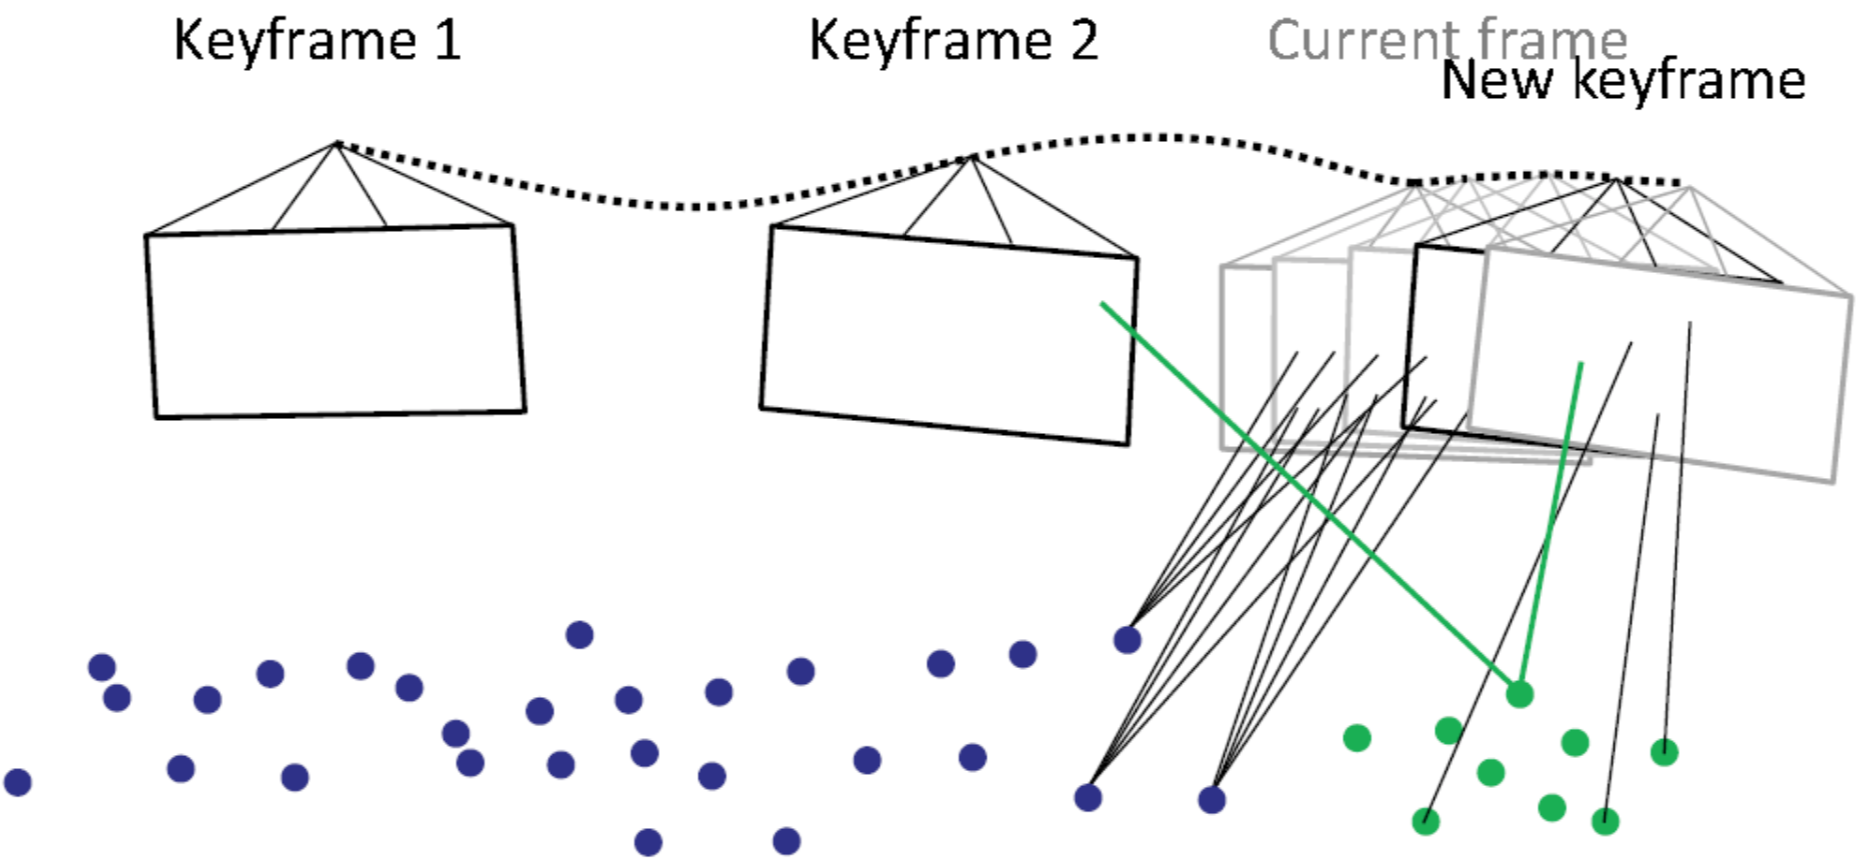
\includegraphics[width=.80\linewidth]{images/framework.png}
	\caption{The PTAM-ORB-SLAM framework}
	\label{fig:framework}
\end{figure}

PTAM represents a multi-threaded key frame based on SLAM.
And ORB\cite{rublee2011orb} features are used for key point detection and matching. Besides, simultaneous localization and mapping (SLAM) is the computational problem of constructing or updating a map of an unknown environment while simultaneously keeping track of an agent's location within it. 
In our project, we extract the key idea of SLAM to estimate the 3D key points.

The key step of 3D reconstruction is the triangulation\cite{hartley1997triangulation}.
Generally, the configuration contains two sensors.
The projection centers of the sensors and the point on the object's surface can define a triangle.
Within this triangle, the distance between the sensors must be known.
Determining the angles between the sensors, the intersection point and the 2D coordinate can be calculated.

Also, the 3D estimate process may not be accurate enough, thus we apply another key step: Bundle Adjustment\cite{triggs1999bundle}.
It can optimize the rough solution given by triangulation.
However, bundle adjustment is solving a nonlinear least square problem, thus takes much longer time.
Luckily, the PTAM framework is designed to mitigate this problem.
It creates a new thread for bundle adjustment, enabling the system to estimate extrinsic metrics in real-time.

In this project, we combine all the knowledge and build an AR system based on these knowledge.
In section \ref{background}, we introduced some basic background knowledge, including ORB, SLAM, Bundle Adjustment and Canny algorithm.
In section \ref{implementation}, some implementation details of this project is elaborated.
And in section \ref{discussion}, we summarize our project and propose some further possible improvement.

\newpage
\section{Background Knowledge}\label{background}

\subsection{Camera Matrix}
For each camera, there is a translation function between the 2D coordinates in the camera scene and the 3D coordinate in the real world. This translation function can be presented as the camera matrix. The general form of camera matrix C is as follows:
$$\lambda\begin{bmatrix}u \\ v \\ 1\end{bmatrix}=
\begin{bmatrix}C_{11} & C_{12} & C_{13} & C_{14}\\
C_{21} & C_{22} & C_{23} & C_{24}\\
C_{31} & C_{32} & C_{33} & C_{34}\end{bmatrix} 
\begin{bmatrix}x \\ y \\ z\\ 1\end{bmatrix} $$
\indent And the matrix C can be divided into two parts, the intrinsic matrix, which is a $3\times 3$ matrix, and the extrinsic matrix, which is a $3\times 4$ matrix\cite{Hartley2004}. The general form is as follows.
$$\begin{bmatrix}C_{11} & C_{12} & C_{13} & C_{14}\\
C_{21} & C_{22} & C_{23} & C_{24}\\
C_{31} & C_{32} & C_{33} & C_{34}\end{bmatrix} = 
\begin{bmatrix}
f_x & \gamma & \delta_x\\
0 & f_y & \delta_y\\
0 & 0 & 1\end{bmatrix}
\begin{bmatrix}r_{11} & r_{12} & r_{13} & t_{1}\\
r_{21} & r_{22} & r_{23} & t_{2}\\
r_{31} & r_{32} & r_{33} & t_{3}\end{bmatrix}$$
\indent With the intrinsic matrix and the extrinsic matrix, we can project any 3D points back to 2D. However, it is not possible to project a 2D point to an exactly 3D point. What we can project by a 2D point is just a 3D line. If we want the exact coordinate of the 3D point, a practical way is to use two cameras and do triangulation.\\
\indent Usually the intrinsic matrix and the extrinsic matrix should be estimated by camera calibration, which usually needs a chess board to represent some points with fixed distance. 
Luckily, in our project, we can get the matrices directly from the IOS system by developing based on Apple's ARKit.

\subsection{SLAM}
Simultaneous localization and mapping (SLAM) is the computational problem of constructing or updating a map of an unknown environment while simultaneously keeping track of an agent's location within it.
Given a series of sensor observations $o_{t}$ over discrete time steps $t$, the SLAM problem is to compute an estimate of the agent's location $x_{t}$ and a map of the environment $m_{t}$. All quantities are usually probabilistic, so the objective is to compute:
$$P(m_{t},x_{t}|o_{1:t})$$
\indent Till now, SLAM is still an active research area.
A SLAM system can be viewed as a combination of mapping, sensing, Kinematics modeling and many other aspects. 
And it may face problems like multiple objects, moving objects and loop closure. 
Also, SLAM algorithms are limited by computational complexity in embedded systems and robots.\\
\indent In our project, we will use a PTAM-ORB-SLAM framework to do the SLAM work. It is an algorithm based on ORB feature and PTAM method. We implemented our augment reality system on a computer with a powerful CPU so we have enough computation resource.

\subsection{Bundle Adjustment}
Given a set of images depicting a number of 3D points from different viewpoints, bundle adjustment can be defined as the problem of simultaneously refining the 3D coordinates along with the parameters of the relative motion, and the optical characteristics of the cameras.
It refines a visual reconstruction to produce jointly optimal 3D points and parameters.
When we assume the intrinsic matrices of different frames stay invariable, bundle Adjustment can be simplified to just optimize the 3D points and the the extrinsic matrix for each frame. 

It means to find the set of parameters that most accurately predict the locations of the observed points in the available images. 
So bundle adjustment is usually achieved by minimizing the re-projection error between the observed 2D points and the predicted 2D points, using nonlinear least-squares algorithms.

Assume that $n$ 3D points are seen in $m$ views and let $x_{ij}$ be the projection of the $i$th point on image $j$.
Let $v_{ij}$ denotes the binary variable that equals $1$ if point $i$ is visible in image $j$ and $0$ otherwise.
The re-projection error can be specified as:
\begin{align*}
    \min_{a_j, b_i}\sum_{i=1}^n\sum_{j=1}^m v_{ij} d(\mathbf{Q}(\mathbf{a_j}, \mathbf{b_i}), x_{ij})^2
\end{align*}
where vector $\mathbf{a_j}$ expresses the extrinsic parameters and each 3D point is parameterized by a vector $\mathbf{b_i}$.
And $\mathbf{Q}(\mathbf{a_j}, \mathbf{b_i})$ is the predicted projection of point $i$ on image $j$, while the $d(\mathbf{x}, \mathbf{y})$ denotes the Euclidean distance between $x$ and $y$.

In order to minimize the sum of the errors, non-linear least squares algorithm\cite{gill1978algorithms} is applied. The fitting is a maximum likelihood estimation of the fitted parameters. There are four popular techniques for non linear least square optimization: Gradient Descent Mehod, Newton-Rhapson Method, Gauss-Newton Method, Levenberg-Marquardt Method.

\subsection{Canny Edge Detector}
The canny edge detector\cite{canny1986computational} is an edge detection operator that uses a multi-stage algorithm to detect edges in images.
Canny edge detection is a technique to extract useful structural information from different vision objects and also reduces useless information.
Among the edge detection methods so far, Canny edge detection algorithm is one of the most reliable and popular detection algorithms.

The process of Canny edge detection algorithm is elaborated as follows\cite{moeslund2009canny}.
\begin{enumerate}
    \item Apply Gaussian filter to smooth the image so that remove the noise;
    \item Find the intensity gradients of the image;
    \item Apply non-maximum suppression to get rid of spurious response to edge detection;
    \item Apply double threshold to determine potential edges;
    \item Finalize the edges by suppressing some weak edges that are not connected to strong edges.
\end{enumerate}

\subsection{Homography}
Homography\cite{berger2009geometry} is a technology that project a plane to another plane. It can be represented by a homography matrix, which is a $3\times 3$ matrix with 8 free parameters. The general form of homography with homography matrix is as follows.
$$\lambda\begin{bmatrix}x' \\ y' \\ 1\end{bmatrix}=
\begin{bmatrix}h_{11} & h_{12} & h_{13}\\
h_{21} & h_{22} & h_{23}\\
h_{31} & h_{32} & h_{33}\end{bmatrix} 
\begin{bmatrix}x \\ y \\ 1\end{bmatrix} $$
\indent Practically, the homography matrix will hardly be given and usually needs to estimate. If we have a set of matching points in the two 2D coordinates, we can have the following equation.
$$\begin{bmatrix}
0 & 0 & 0 & -u_1 & -v_1 & -1 & y_1u_1 & y_1v_1 & y_1\\
u_1 & v_1 & 1 & 0 & 0 & 0 & -x_1u_1 & -x_1v_1 & -x_1\\
0 & 0 & 0 & -u_2 & -v_2 & -1 & y_2u_2 & y_2v_2 & y_2\\
u_2 & v_2 & 1 & 0 & 0 & 0 & -x_2u_2 & -x_2v_2 & -x_2\\
\vdots & \vdots & \vdots & \vdots & \vdots & \vdots & \vdots & \vdots & \vdots\\
0 & 0 & 0 & -u_N & -v_N & -1 & y_Nu_N & y_Nv_N & y_N\\
u_N & v_N & 1 & 0 & 0 & 0 & -x_Nu_N & -x_Nv_N & -x_N\\
\end{bmatrix}
\begin{bmatrix}
h_{11} \\ h_{12} \\ h_{13} \\ 
h_{21} \\ h_{22} \\ h_{23} \\ 
h_{31} \\ h_{32} \\ h_{33} 
\end{bmatrix}
=\begin{bmatrix}
0 \\ 0 \\ \vdots \\ 0 \\
\end{bmatrix}$$
\indent Since the homography matrix has 8 free parameters, the least amount of pairs of points needed to solve the equation is 4. If we have only four points, one method to solve it is to use Rayleigh Quotient\cite{horn1985cr}, which is in the following form:
$$\arg \min_h \frac{h^TA^TAh}{h^Th}$$
\indent And one way to solve that is to use steepest descent.\\
\indent If we have more than three points, then the rank of the first matrix A is 9, so we can use SVD decomposition to get the best approximation of H, which is the eigenvector with the least eigenvalue.

\newpage
\section{Implementation Details}\label{implementation}

\subsection{Pipeline}
Our pipeline contains several steps: 
\begin{enumerate}
    \item Record video and intrinsic matrix of camera; 
    \item Extract key points based on orb feature extractor; 
    \item Match key points using KNN method; 
    \item Pick up key frames according to distances; 
    \item Reconstruct 3D cloud points using triangulation; 
    \item Use bundle adjustment to optimize projection matrix and 3D points; 
    \item Project virtual television to the surface. 
\end{enumerate}
The project is basically implemented using C++ and based on some open-source libraries like opencv\cite{itseez2015opencv} and ceres-solver\cite{ceres-solver}.

\subsection{Extract key points with ORB}
The first step of SLAM is to find the key points in each frame. In our implementation , we use ORB descriptor to do that job. ORB is basically a fusion of FAST\cite{rosten2006machine} keypoint detector and BRIEF\cite{calonder2010brief} descriptor with many modifications to enhance the performance. However, dislike FAST and BRIEF descriptor, ORB is invariant to rotation and resistant to noise.\\
\begin{figure}[h]
	\centering
	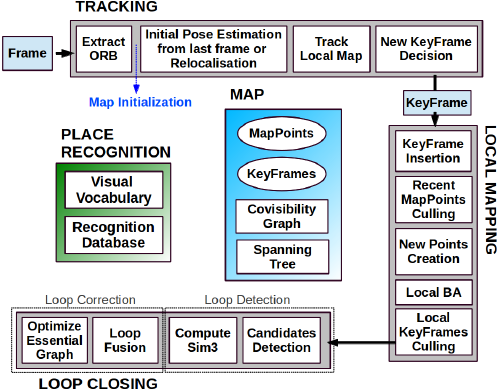
\includegraphics[width=.80\linewidth]{images/orb.png}
	\caption{The ORB framework}
	\label{fig:framework}
\end{figure}
\indent ORB uses FAST to find the key points. It also uses pyramids to product multi-scale features. To achieve rotation invariant, it computes the intensity weighted centroid of the patch and get the orientation from it. For further improvement, moments are computed with x and y which should be in a circular region of radius $r$, where $r$ r is the size of the patch.\\
\indent As for descriptors, ORB use BRIEF descriptors, but with amelioration. ORB steers BRIEF according to the orientation of key points. ORB uses the orientation of patch , $\theta$, to compute the rotation matrix, and rotate every point in the patch accordingly. The angle is discretized into 12 degrees (by increments of $30^\circ$). ORB will use the rotated pre-computed BRIEF patterns as the feature descriptor.\\
\indent Additionally, Our ORB implementation tries to maintain the high variance of BRIEF in the ORB descriptor, which is destroyed by the rotation. High variance makes a feature more discriminative, since it responds differently to inputs. Another desirable property is to have the tests uncorrelated, since then each test will contribute to the result. To resolve all these, our ORB implementation runs a greedy search among all possible binary tests to find the ones that have both high variance and means close to 0.5, as well as being uncorrelated.

\subsection{Match key points by KNN}
When a new frame comes, we will first compute out the ORB features of it. Then, we will compare the features of the key points with those of the former frame. The matching algorithm we use is K-Nearest Neighbours algorithm\cite{altman1992introduction}.\\
\indent Since the ORB feature is a binary feature, the distance between two ORB features can be represented by the differences in bits. We wrote a score function about it to score the similarity of two ORB features.\\
\indent With KNN algorithm, we will find the K nearest neighbours of every key point in the current frame. 
In our case, K equals two. We compare the score of the first and the second nearest points. If the score of the nearest point is two times higher than the score of the second nearest point, then we consider the matching is 'valid'. This step is necessary because if we don't do that, we will have many mismatches by several similar key points.

\subsection{Pick up key frames}
In our implementation of SLAM, we do not save the information of every frame for storage consideration. So it is important to judge which frames to store. We denote the frames we store as key frames.\\
\indent The first frame must be the key frame, since it contains our initial information. For any following frame, we will compute the distance of the frame to the last key frame. The distance is defined by the difference between their distances to the camera scene. And their distance to the camera scene is defined by the average value of the key points in 'z' coordinate.\\
\indent Intuitively, if the current frame is too far away from the last key frame, then we denote it as the new key frame. Therefore, we will not meet too much accumulation error by the long series of frames.

\subsection{Reconstruct 3D cloud points}
The next step of SLAM is to reconstruct the 3D cloud points of the key points. The method we implement here is triangulation.\\
\begin{figure}[h]
	\centering
	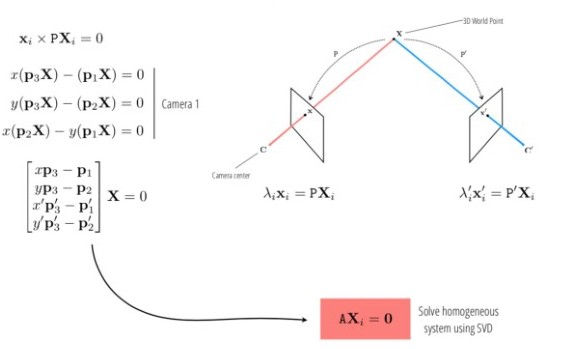
\includegraphics[width=.80\linewidth]{images/triangulation.jpg}
	\caption{Triangulation}
	\label{fig:framework}
\end{figure}\\
\indent For each frame, we do triangulation between that frame and the last key frame. Since the distance between them will not be very large according to our key frame picking up method, so probably there will be a fair amount of matching points.\\
\indent For each pair of matching points, we can have the equation as shown in the picture.
$$\begin{bmatrix}
xp_3-p_1 \\ yp_3 - p_2 \\ x'p_3' - p_1' \\ y'p_3' - p_2'
\end{bmatrix} X = 0$$
\indent Then we can solve this equation by SVD decomposition, which will give us the 3D coordinate of X. With multiple pairs of matched points, we will get a point cloud of all the key points.

\subsection{Bundle Adjustment}
We use ceres-solver to achieve non-linear least square optimization.
It is an open source C++ library for modeling and solving large, complicated optimization problems, especially useful for solving non-linear least squares problems.

In our project, we choose to optimize each three successive key frames.
Given each intrinsic and extrinsic matrices as well as the observed 2D points and estimated 3D points, the bundle adjustment function will return the optimized 3D points along with the extrinsic matrices of the last two frames.
Here we assume the intrinsic matrix does not change in all frames and in each three frames, the extrinsic matrix of the first frame has highest accuracy and will keep unchangeable.

In detail, we know the extrinsic matrix is combined by the rotation matrix of $3\times3$ and a translation matrix of $3\times1$. Firstly, we used Rodrigues' rotation formula \cite{rodrigues1840lois} to transform the rotation matrix to a rotation vector of 3 elements.
The reason is that there are subject to 6 norm and orthogonality constraints in the rotation matrix so that it only has 3 degrees of freedom.
In the optimization problem, redundancy is not preferable and should be removed.
After transformation, the extrinsic matrix can be expressed as 6 elements.

For example, if we got $N$ points, to take the gradient of the function with the implementation of dual numbers, the ceres-solver tends to create a template contains $N\times3+6\times(3-1)$ variables to optimize.

Since ceres-solver allows automatic differentiation, it is convenient to use it to achieve bundle adjustment in another thread.
Besides, we choose sparse normal cholesky as the linear solver type, for our Jacobian matrix can be sparse.


\subsection{Projection to the plane}
The last part of our project is to project the TV frames to the camera scene. It is actually done in two steps: first project it to the 3D coordinate, and then project it back to the 2D camera scene.\\
\indent There is one thing that need to be done before the projection. That is to figure out the plane where the visual television should be put on. In implementation, we will deliver four 3D points to this part as the four corners of the visual television in the 3D world. Mention that these four points may not be exactly on the same plane (although they should be), so approximation is required to get the plane we want. Denote the function of the plane is $Ax+By+Cz+D = 0$, then we have the following equation.
$$\begin{bmatrix}
x_1 & y_1 & z_1 & 1\\
x_2 & y_2 & z_2 & 1\\
x_3 & y_3 & z_3 & 1\\
x_4 & y_4 & z_4 & 1\end{bmatrix}
\begin{bmatrix}A \\ B \\ C \\ D\end{bmatrix} 
\approx \begin{bmatrix}0 \\ 0 \\ 0 \\ 0
\end{bmatrix} $$
\indent The best approximation with least square error of the parameters of the plane is the eigenvector with the least eigenvalue of the first $4 \times 4$ matrix.\\
\indent After achieving the plane, we also need to decide the direction that we put the visual television on. In our project, we assume that the direction is the same as the normal vector of the plane we approximated. And we will do normalization to that vector to let the length of it to be 1 and let its value on z-coordinate to be negative, which leads the visual television to be towards us rather than opposite us.\\
\indent The third step in this part is to project the 3D points into 2D. With the intrinsic and extrinsic matrix, it can be done by directly multiple these two matrixes with the 3D coordinate. The equation is as follows.
$$\lambda\begin{bmatrix}u \\ v \\ 1\end{bmatrix} = 
\begin{bmatrix}
f_x & \gamma & \delta_x\\
0 & f_y & \delta_y\\
0 & 0 & 1\end{bmatrix}
\begin{bmatrix}r_{11} & r_{12} & r_{13} & t_{1}\\
r_{21} & r_{22} & r_{23} & t_{2}\\
r_{31} & r_{32} & r_{33} & t_{3}\end{bmatrix}
\begin{bmatrix}
x \\ y \\ z \\ 1
\end{bmatrix}$$
\indent The last step of projection is homography. The reason to do that is that it is too computational expensive to project every point to 3D and then back to 2D. In our implementation, we recognize the visual television as an assemble of plane rather than a set of 3D points. Therefore, to draw the television on the camera scene, what we do is to project plane to plane rather than project point to point. The method of applying homography is included in the background knowledge part. One thing need to mention is order of which plane to project first. We assume that all the four border of the visual television are of the same color, so the order of projecting border does not make any difference. The only thing we have to pay attention to is to project the television frame in the last step.

\newpage
\section{Results}

In Figure \ref{fig:original}, we present a frame image of the input video which is picked randomly.
\begin{figure}[h]
	\centering
	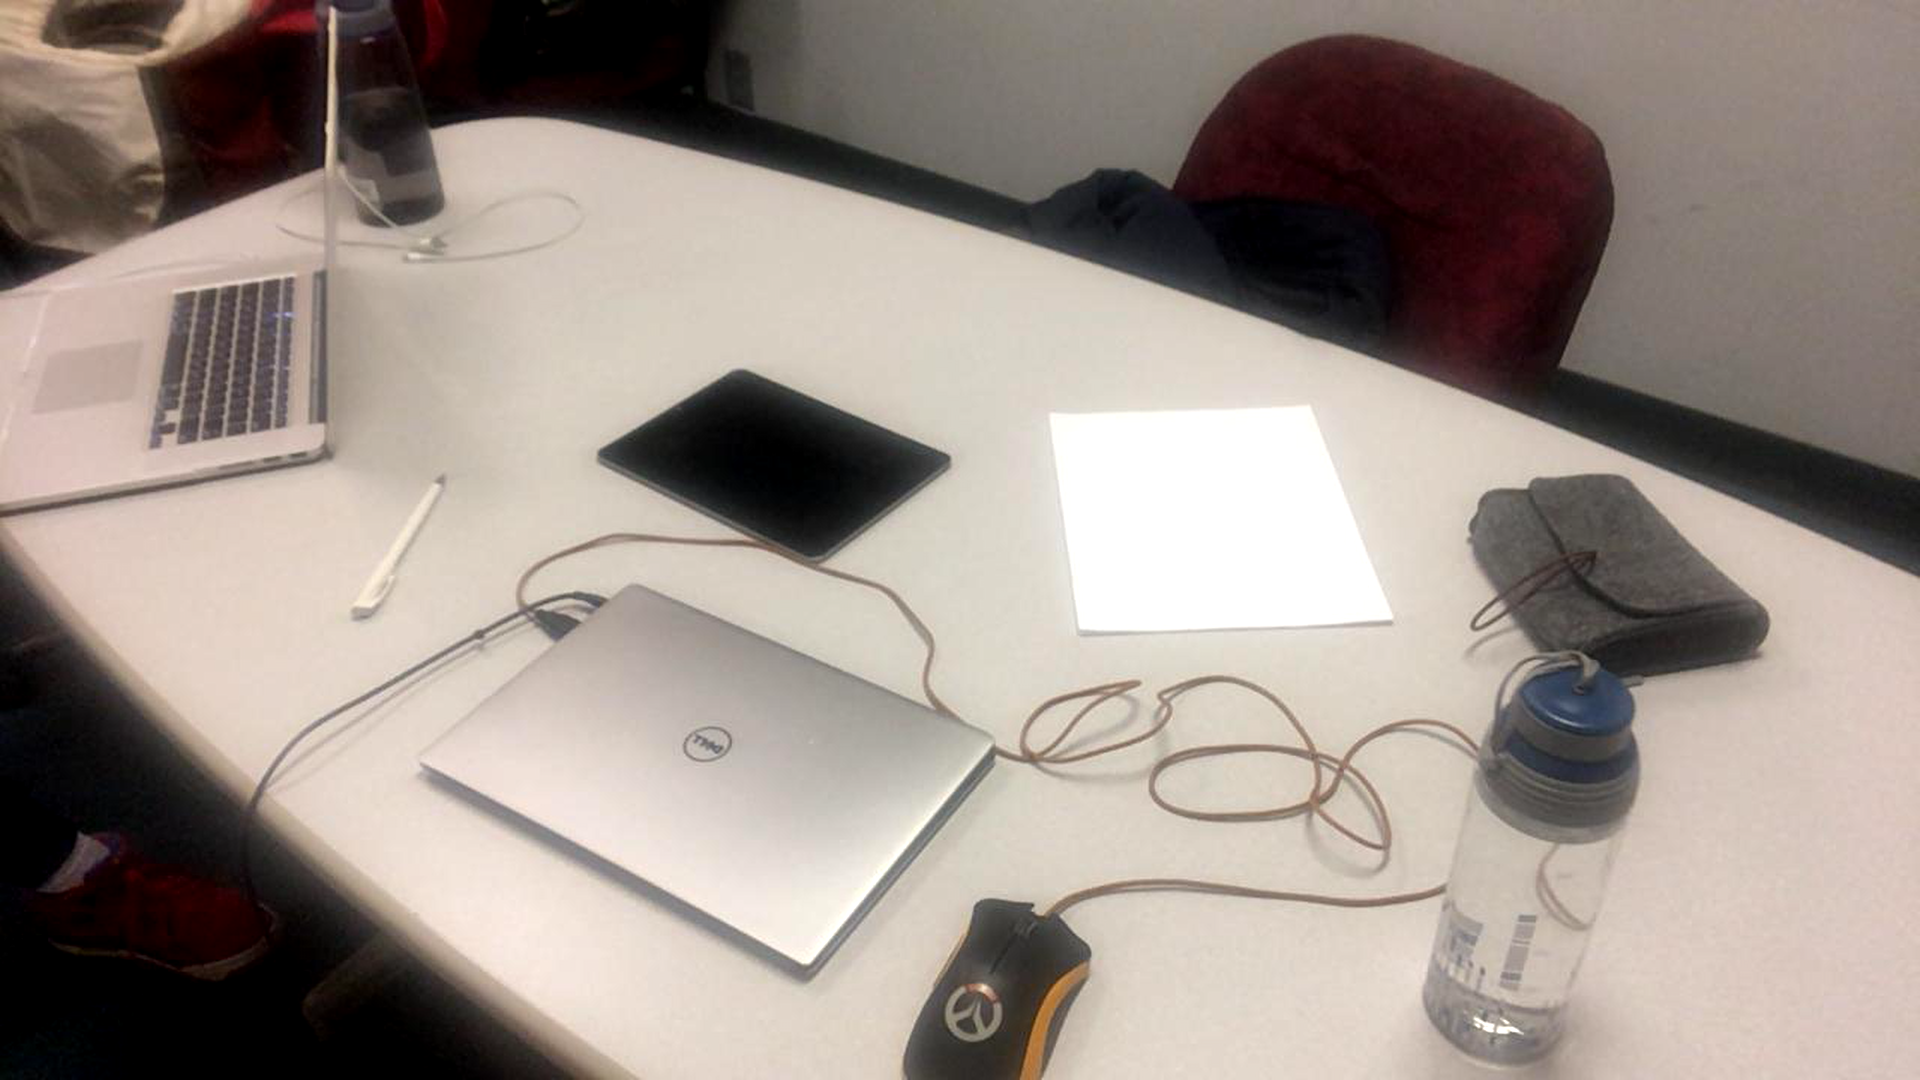
\includegraphics[width=.80\linewidth]{images/original.png}
	\caption{One frame image of the input video}
	\label{fig:original}
\end{figure}

The results are of two parts.
One direct result is after using the canny edge detector.
The result is shown in Figure \ref{fig:canny}.
\begin{figure}[h]
	\centering
	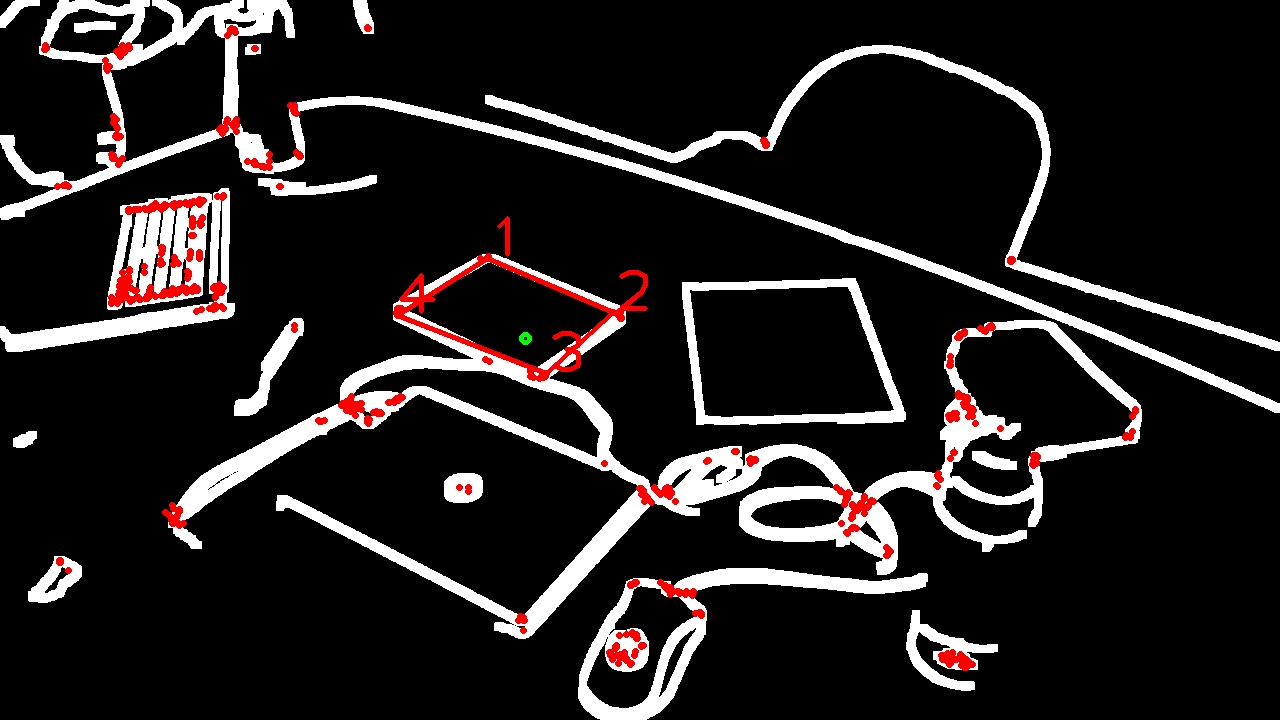
\includegraphics[width=.80\linewidth]{images/canny.jpeg}
	\caption{The Result Using Canny Edge Detector.}
	\label{fig:canny}
\end{figure}

It could be regarded as one pre-processing step to help us find the plane to project our prepared video onto.
We can see in the result that our system can find four proper edges which can form the plane.

As our system runs, the prepared video can be successfully projected onto the plane we just found.
And one frame of our final result is shown in Figure \ref{fig:final}.
\begin{figure}[h]
	\centering
	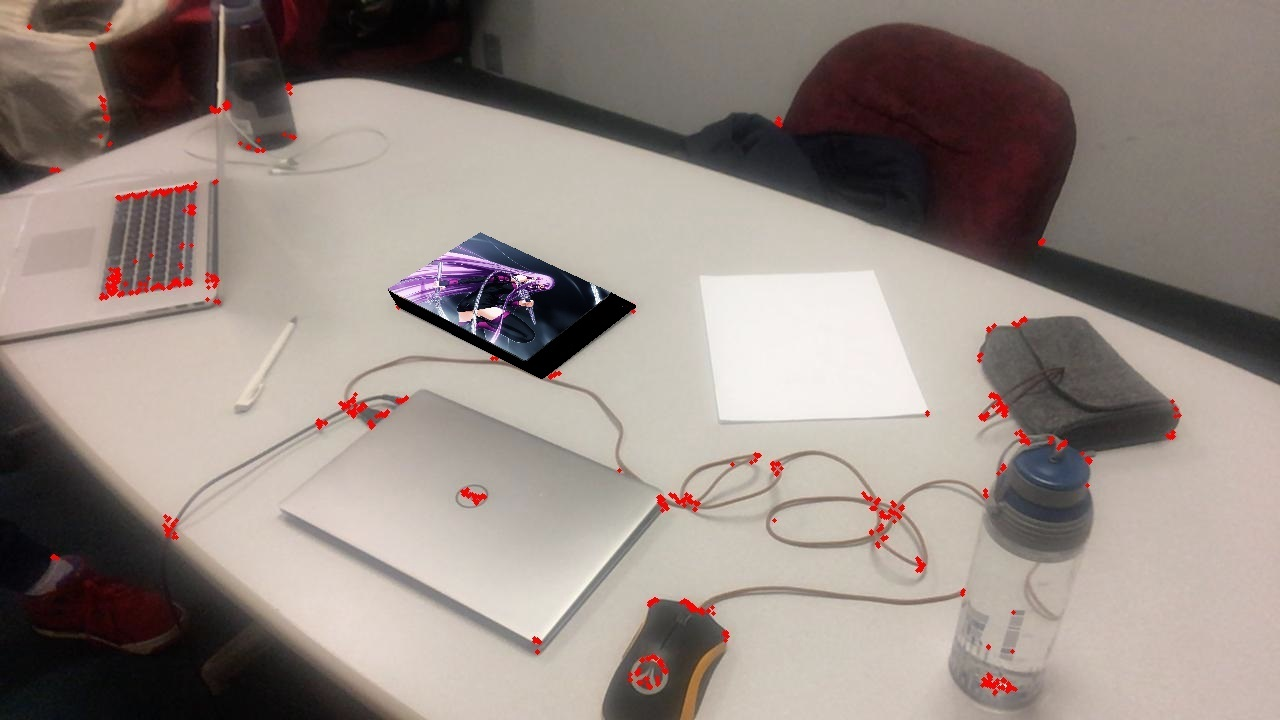
\includegraphics[width=.80\linewidth]{images/final.jpeg}
	\caption{One frame of final result.}
	\label{fig:final}
\end{figure}

\newpage
\section{Discussion}\label{discussion}
Our project is a complex system which involves key point detection, feature matching, key frame storing, bundle adjustment and image projection. However, there are still some aspects we hope to further implement and some attributes that we hope to achieve.

The first thing is that we hope to recognize a white wall and project the television on it. However, in our experiments, it seems impossible to project a stable visual television on a pure background because of lack of key points. In general AR industry, it actually is a knotty problem to do SLAM in pure background. But we think there is a way to solve this problem from another aspect. We suppose we could use the gyroscope in our mobile phones to do that job. We could assume that the camera intrinsic does not change in front of a pure background, and we can calculate the extrinsic by the results given by gyroscope. With these information, we can fix a 3D point as the center of the visual television, and fix a vector as the direction of the television from the first frame. In the following frames, we just need to draw the visual television according to the 3D coordinates regardless of whether there are any key points in the real scene.

The second thing is about computational limitation. Our project is implemented on a personal computer. However, if want it to be a real product, it should be installed in a mobile device. As we all know, the computation ability of a mobile device is far weaker than a computer. So we need to do some additional acceleration for it. One part we can do amelioration is the feature matching part. In our implement, we compute the score between every key point in the current frame with every key point in the last key frame, which contain much redundant computation. In reality, the correct match for one point would not be far away from its current location. So if we do local approximation first and then do matching, a lot of computation will be saved while the performance will not be harmed.

The third thing is the recognition of the scene. In our implement, we always match the current frame with the last key frame. However, if we see the same scene or the same object twice, we will not recognition it as the thing we have seen. On the contrary, we re-compute every point as totally new points, which generates both redundant computation and accumulation error. For further improvement, we hope to add a recognition part to match the scene we are looking at now and we seen before. If two scenes or two objects are matched, we hope to refine the location by merging the two sets of coordinates.

\newpage
\begin{spacing}{1.0}
%%行间距变为single-space
\bibliographystyle{plain}
\bibliography{references}
\end{spacing}

%%% End document
\end{document}